\documentclass[a4paper, 12pt]{article}
\usepackage[utf8]{inputenc}

\usepackage[a4paper,top=1.3cm,bottom=2cm,left=1.5cm,right=1.5cm,marginparwidth=0.75cm]{geometry}
\usepackage{cmap}				
\usepackage{mathtext} 				
\usepackage[T2A]{fontenc}			
\usepackage[utf8]{inputenc}			
\usepackage[english,russian]{babel}	
\usepackage{multirow}
\usepackage{mathtools}
\mathtoolsset{showonlyrefs=true}

\usepackage{graphicx}
\usepackage{wrapfig}
\usepackage{tabularx}
\usepackage{caption}

\title{2.1.3-theory}
\author{Влад Черниенко}
\date{March 2022}

\begin{document}

    \begin{titlepage}
    
        \begin{center}
            {\large МОСКОВСКИЙ ФИЗИКО-ТЕХНИЧЕСКИЙ ИНСТИТУТ (НАЦИОНАЛЬНЫЙ ИССЛЕДОВАТЕЛЬСКИЙ УНИВЕРСИТЕТ)}
        \end{center}
        \begin{center}
            {\large Фихтех-школа радиотехники и компьютерных технологий}
        \end{center}
        
        \vspace{4.5cm}
        
        {\huge
            \begin{center}
                {\bf Лабораторная работа 2.2.3}\\
                Измерение теплопроводности воздуха при атмосферном давлении
            \end{center}
        }
        
        \vspace{10cm}
        
        \begin{flushright}
            {\LARGE Автор: \\ Черниенко Владислав Антонович \\ \vspace{0.2cm} Группа Б01-110}
        \end{flushright}
        
    \end{titlepage}
    
    
    \noindent {\bf Цель работы:} измерить коэффициент теплопроводности воздуха при атмосферном давлении в зависимости от температуры.\\
    
    \noindent {\bf В работе используются:} цилиндрическая колба с натянутой по оси нитью; термостат; вольтметр и амперметр (цифровые мультиметры); эталонное сопротивление; источник постоянного напряжения; реостат (или магазин сопротивлений).\\
    
    \begin{center}
        {\Large {\bf Теоретические сведения}}
    \end{center}
    
    \textit{Теплопроводность} — это процесс передачи тепловой энергии от нагретых частей системы к холодным за счёт хаотического движения частиц среды (молекул, атомов и т.п.). В газах теплопроводность осуществляется за счёт непосредственной передачи кинетической энергии от быстрых молекул к медленным при их столкновениях. Перенос тепла описывается законом Фурье, утверждающим, что плотность потока энергии $ \vec{q} $ $ [\frac{\text{Вт}}{\text{м}^2}] $ (количество теплоты, переносимое через единичную площадку в единицу времени) пропорциональна градиенту температуры $ \nabla T $:
    \begin{equation}
        \vec{q}=-k \cdot \nabla T,
        \label{first}
    \end{equation}
    где $ k $ $ [\frac{\text{Вт}}{\text{м} \cdot \text{К}}] $ — \textit{коэффициент теплопроводности}.
    
    Молекулярно-кинетическая теория даёт следующую оценку для коэффициента теплопроводности газов:
    \begin{equation}
        k \sim \lambda\bar{v} \cdot nc_{V},
        \label{second}
    \end{equation}
    где $ \lambda $ — длина свободного пробега молекул газа, $ \bar{v} = \sqrt{\frac{8 k_{\text{Б}} T}{\pi m}} $ — средняя скорость их теплового движения, $ n $ — концентрация (объёмная плотность) газа, $ c_{V} = \frac{i}{2} k_{\text{Б}} $ — его теплоёмкость при постоянном объёме в расчёте на одну молекулу ($ i $ — эффективное число степеней свободы молекулы).
    
    Длина свободного пробега может быть оценена как $ \lambda = 1/n\sigma $, где $ \sigma $ — эффективное сечение столкновений молекул друг с другом. Тогда из \eqref{second} видно, что коэффициент теплопроводности газа не зависит от плотности газа и \textit{определяется только его температурой}. В простейшей модели твёрдых шариков $ \sigma = const $, и коэффициент теплопроводности пропорционален корню абсолютной температуры: $ k \propto \bar{v}/\sigma \propto \sqrt{T} $.
    
    \begin{wrapfigure}{r}{5cm}
        \center{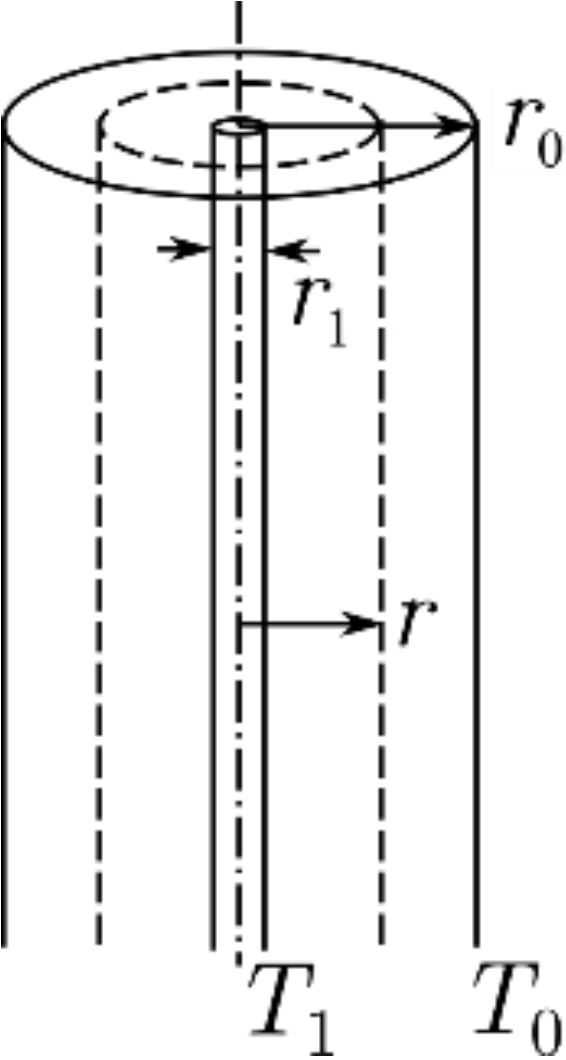
\includegraphics[width=3cm]{images/1.png}}
        \caption{Геометрия задачи}
        \label{pic1}
    \end{wrapfigure}
    Рассмотрим стационарную теплопроводность в цилиндрической геометрии (см. рис. \ref{pic1}). Пусть тонкая нить радиусом $ r_{1} $ и длиной $ L $ помещена на оси цилиндра радиусом $ r_{0} $. Температура стенок цилиндра $ T_{0} $ поддерживается постоянной. Пусть в нити выделяется некоторая тепловая мощность $ Q $ [Вт]. Если цилиндр длинный ($ L \gg r_{0} $), можно пренебречь теплоотводом через его торцы. Тогда все параметры газа можно считать зависящими только от расстояния до оси системы $ r $. Вместо \eqref{first} имеем
    \begin{equation}
        q = -k \frac{dT}{dr}.
        \label{third}
    \end{equation}
    В \textit{стационарном} состоянии полный поток тепла через любую цилиндрическую поверхность радиуса $ r $ площадью $ S = 2 \pi r L$ должен быть одинаков и равен $ Q = q S $:
    \begin{equation}
        Q = -2 \pi r L \cdot k \frac{dT}{dr} = const.
        \label{fourth}
    \end{equation}
    Если перепад температуры $ \Delta T = T_{1} - T_{0} $ между нитью и стенками цилиндра мал ($ \Delta T \ll T_{0} $), то в \eqref{fourth} можно пренебречь изменением теплопроводности от температуры в пределах системы, положив $ \kappa \approx \kappa (T_{0}) $. Тогда разделяя переменные в \eqref{fourth} и интегрируя от радиуса нити до радиуса колбы, получим
    \begin{equation}
        Q = \frac{2 \pi L}{ln \frac{r_{0}}{r_{1}}}k \cdot \Delta T.
        \label{fifth}
    \end{equation}
    Видно, что поток тепла через систему пропорционален разности температур в ней (\textit{закон Ньютона}).\\
    
    \begin{center}
        {\Large {\bf Экспериментальная установка}}
    \end{center}
    
    \begin{wrapfigure}{r}{6cm}
        \center{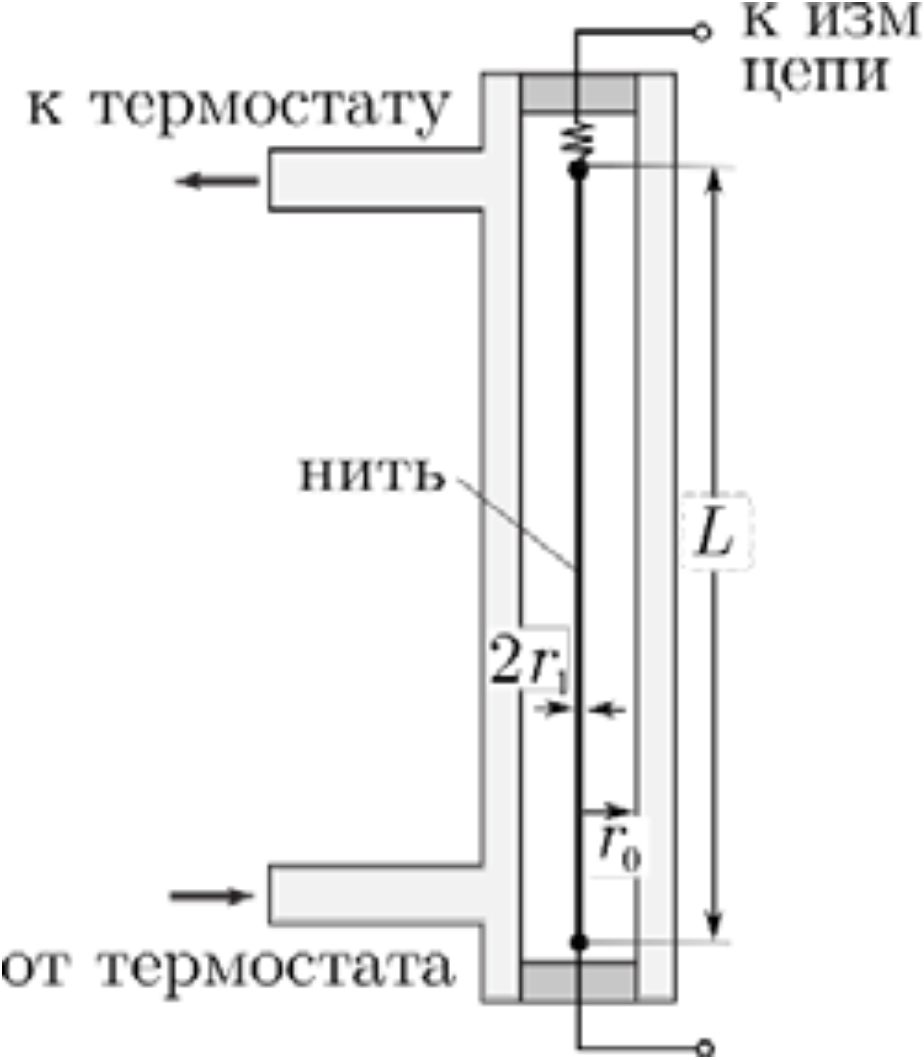
\includegraphics[width=1\linewidth]{images/2.png}}
        \caption{Схема установки}
        \label{pic2}
    \end{wrapfigure}
    Схема установки приведена на рис. \ref{pic2}. На оси полой цилиндрической трубки с внутренним диаметром $ 2r_{0} \sim 1 \text{ см} $ размещена металлическая нить диаметром $ 2r_{1} \sim 0,05 \text{ мм} $ и длиной $ L \sim 40 \text{ см} $ ( материал нити и точные геометрические размеры указаны в техническом описании установки). Полость трубки заполнена воздухом (полость через небольшое отверстие сообщается с атмосферой). Стенки трубки помещены в кожух, через которых пропускается вода из термостата, так что их температура $ t_{0} $ поддерживается постоянной. Для предотвращения конвекции трубка расположена вертикально.
    
    Металлическая нить служит как источником тепла, так и датчиком температуры (термометром сопротивления). По пропускаемому через нить постоянному току $ I $ и напряжению $ U $ на ней вычисляется мощность нагрева по закону Джоуля-Ленца:
    \begin{equation}
        Q = UI,
    \end{equation}
    и сопротивление нити по закону Ома:
    \begin{equation}
        R = \frac{U}{I}.
    \end{equation}
    
    На рис. \ref{pic3} приведена электрическая схема установки. Эта схема предусматривает использование одного вольтметра и эталонного сопротивления $ R_{э} \sim 10 \text{ Ом} $, включённого последовательно с нитью. В положении переключателя 2 вольтметр измеряет напряжение на нити, а в положении 1 — напряжение на $ R_{э} $, пропорциональное току через нить. Для исключения влияния контактов и подводящих проводов эталонное сопротивление $ R_{э} $ необходимо подключать в цепь по четырёхпроводной схеме.
    
    \begin{figure}[h]
        \center{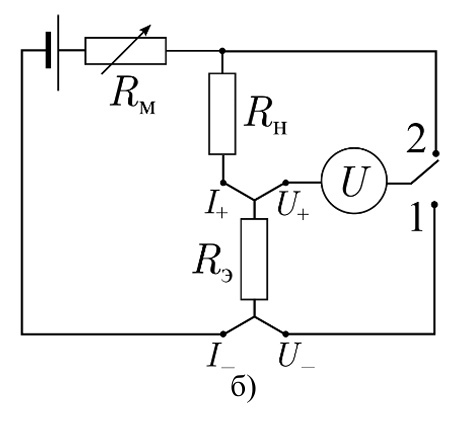
\includegraphics[width=7cm]{images/3.jpg}}
        \caption{Электрическая схема}
        \label{pic3}
    \end{figure}
    
    \newpage
    
    \begin{center}
        {\Large {\bf Ход работы}}
    \end{center}
    
    \begin{enumerate}
    
        \item[1.] Для начала запишем все необходимые параметры установки и погрешности приборов, взятые из технического описания:
        \begin{itemize}
            \item Диаметр нити: $2 r_1 = 0,055 \pm 0,005$ мм
            \item Диаметр колбы: $2 r_0 = 10,0 \pm 0,1$ мм
            \item $ln(r_2 / r_1) \sim 5,30$
            \item Длина нити: $L = 365 \pm 2$ мм
            \item Эталонное сопротивление: $R_э = 10,000$ Ом
            \item ЭДС: $E = 4$ В
            \item Погрешность вольтметра: $\varepsilon_U \sim 0,1$ \%
            \item Погрешность термостата: $\sigma_T = \pm 0,1^\circ C$
        \end{itemize}
        
        \item[2.] Выставим сопротивление на магазине сопротивлений $R_М = 0$ Ом, для того, чтобы рассчитать максимальное количество теплоты, которое может выделиться на нити: $Q_{max} = 386,3$ мВт.
    
        \item[3.] По формуле $Q = \alpha \cdot Q_{max}$ найдём такие сопротивления магазина сопротивлений $R_{М}$, при которых мощность нагрева $Q$ возрастает равномерно в диапазоне от 0 до $Q_{max}$. Результат занесём в табл. \ref{table1}.
        
        \begin{table}[ht]
            \centering
            \begin{tabular}{|c|c|c|c|c|c|c|c|c|c|c|c|}
                \hline
                $\alpha$ & 1 & 0,9 & 0,8 & 0,7 & 0,6 & 0,5 & 0,4 & 0,3 & 0,2 & 0,1 & 0,01 \\
                \hline
                $R_{М}$, Ом & 0 & 1,4 & 3 & 4,9 & 7,3 & 10,4 & 14,5 & 20,6 & 30,9 & 54,1 & 225 \\
                \hline
            \end{tabular}
            \caption{Значения сопротивлений $R_{М}$ магазина сопротивлений}
            \label{table1}
        \end{table}
        
        \item[4.] Выставим значение температуры термостата $T = 22^\circ C$ – комнатная температура. При этой температуре построим нагрузочную кривую $R_н(Q)$:
        
        Будем последовательно менять сопротивление магазина сопротивлений, беря значения $R_М$ из табл. \ref{table1}. Далее будем измерять напряжения на эталонном сопротивлении $R_э$ ($U_1$) и на нити $R_н$ ($U_2$) при определённом значении $R_М$. По этим значениям, будем вычислять мощность нагрева $Q$, а затем и сопротивление нити $R_н$ при данном $R_М$. Результаты будем заносить в табл. \ref{table2}. Также по ходу выполнения работы построим график нагрузочной кривой по МНК.
        
        \item[5.] Проведём измерения нагрузочных кривых согласно п. 3 ещё для 4 температур термостата в диапазоне от 30 до 60$^\circ C$. Построим их графики по МНК. Результаты также будем заносить в табл. \ref{table2}.
        
    \end{enumerate}

    \begin{table}[pt]
    
        \begin{minipage}[ht]{0.47\linewidth}
            \begin{tabular}{|c|c|c|c|c|}
                \hline
                \multicolumn{5}{|c|}{$T = 22^\circ C$} \\
                \hline
                $R_М$, Ом & $U_1$, мВ & $U_2$, мВ & $Q$, мВт & $R_н$, Ом \\
                \hline
                0 & 1560 & 2476 & 386,3 & 15,87 \\
                \hline
                1,4 & 1487 & 2342 & 348,3 & 15,75 \\
                \hline
                3 & 1410 & 2204 & 310,8 & 15,63 \\
                \hline
                4,9 & 1328 & 2060 & 273,6 & 15,51 \\
                \hline
                7,3 & 1236 & 1901 & 235,0 & 15,38 \\
                \hline
                10,4 & 1134 & 1730 & 196,2 & 15,26 \\
                \hline
                14,5 & 1021 & 1543 & 157,5 & 15,11 \\
                \hline
                20,6 & 887,7 & 1330 & 118,1 & 14,98 \\
                \hline
                30,9 & 726,3 & 1079 & 78,37 & 14,86 \\
                \hline
                54,1 & 514,1 & 756,8 & 38,91 & 14,72 \\
                \hline
                225 & 162,6 & 237,4 & 3,860 & 14,60 \\
                \hline
            \end{tabular}
        \end{minipage}
        \hfill
        \begin{minipage}[ht]{0.47\linewidth}
            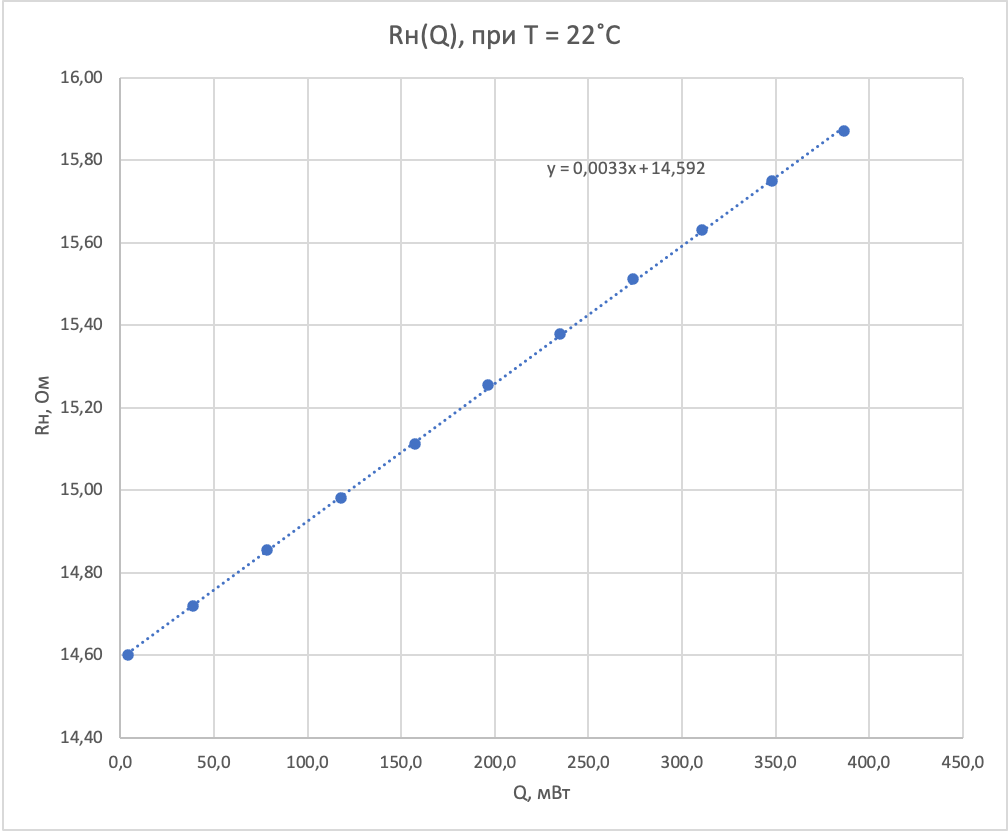
\includegraphics[width=\linewidth]{images/ch1.png}
        \end{minipage}
        
        \vspace{1cm}
        
        \begin{minipage}[ht]{0.47\linewidth}
            \begin{tabular}{|c|c|c|c|c|}
                \hline
                \multicolumn{5}{|c|}{$T = 30^\circ C$} \\
                \hline
                $R_М$, Ом & $U_1$, мВ & $U_2$, мВ & $Q$, мВт & $R_н$, Ом \\
                \hline
                0 & 1540 & 2497 & 384,5 & 16,21 \\
                \hline
                1,4 & 1469 & 2363 & 347,1 & 16,09 \\
                \hline
                3 & 1394 & 2226 & 310,3 & 15,97 \\
                \hline
                4,9 & 1314 & 2083 & 273,7 & 15,85 \\
                \hline
                7,3 & 1224 & 1924 & 235,5 & 15,72 \\
                \hline
                10,4 & 1123 & 1752 & 196,7 & 15,60 \\
                \hline
                14,5 & 1012 & 1566 & 158,5 & 15,47 \\
                \hline
                20,6 & 880,7 & 1352 & 119,1 & 15,35 \\
                \hline
                30,9 & 721,6 & 1098 & 79,23 & 15,22 \\
                \hline
                54,1 & 511,8 & 772,1 & 39,52 & 15,09 \\
                \hline
                225 & 162,3 & 242,9 & 3,942 & 14,97 \\
                \hline
            \end{tabular}
        \end{minipage}
        \hfill
        \begin{minipage}[ht]{0.47\linewidth}
            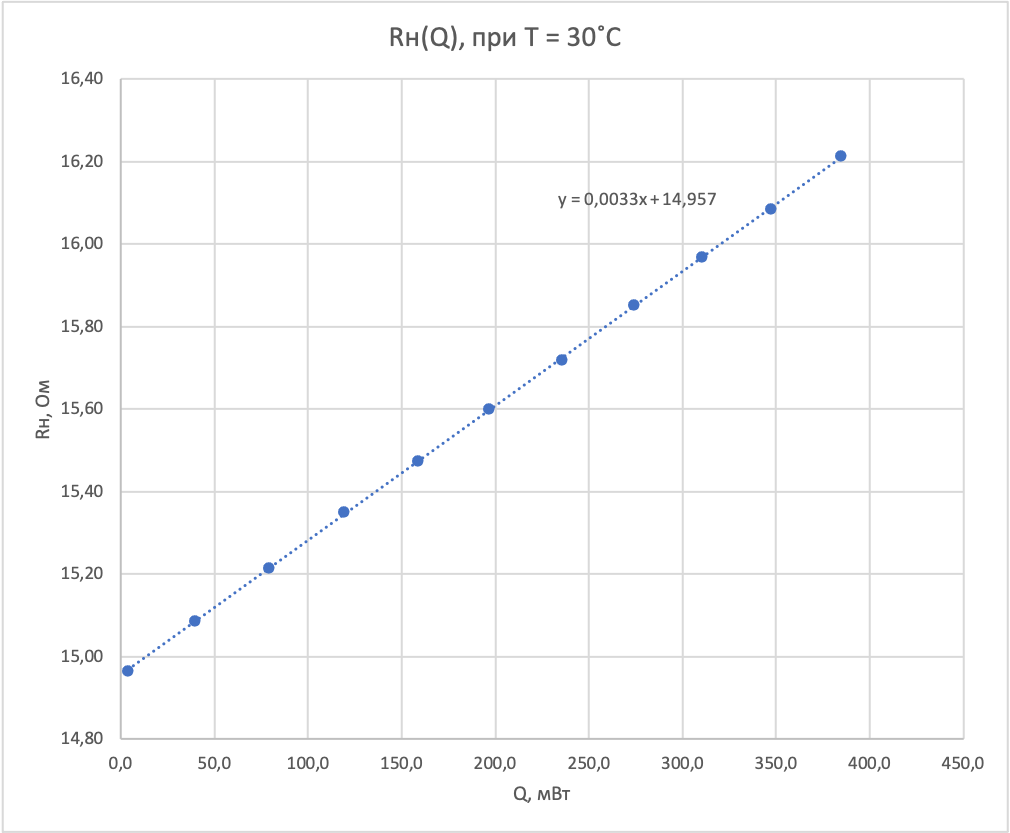
\includegraphics[width=\linewidth]{images/ch2.png}
        \end{minipage}
        
        \vspace{1cm}
        
        \begin{minipage}[ht]{0.47\linewidth}
            \begin{tabular}{|c|c|c|c|c|}
                \hline
                \multicolumn{5}{|c|}{$T = 40^\circ C$} \\
                \hline
                $R_М$, Ом & $U_1$, мВ & $U_2$, мВ & $Q$, мВт & $R_н$, Ом \\
                \hline
                0 & 1516 & 2521 & 382,2 & 16,63 \\
                \hline
                1,4 & 1447 & 2389 & 345,7 & 16,51 \\
                \hline
                3 & 1374 & 2253 & 309,6 & 16,40 \\
                \hline
                4,9 & 1296 & 2110 & 273,5 & 16,28 \\
                \hline
                7,3 & 1208 & 1952 & 235,8 & 16,16 \\
                \hline
                10,4 & 1110 & 1780 & 197,6 & 16,04 \\
                \hline
                14,5 & 1001 & 1593 & 159,5 & 15,91 \\
                \hline
                20,6 & 872,5 & 1377 & 120,1 & 15,78 \\
                \hline
                30,9 & 716,0 & 1121 & 80,26 & 15,66 \\
                \hline
                54,1 & 508,9 & 790,3 & 40,22 & 15,53 \\
                \hline
                225 & 162,0 & 249,7 & 4,045 & 15,41 \\
                \hline
            \end{tabular}   
        \end{minipage}
        \hfill
        \begin{minipage}[ht]{0.47\linewidth}
            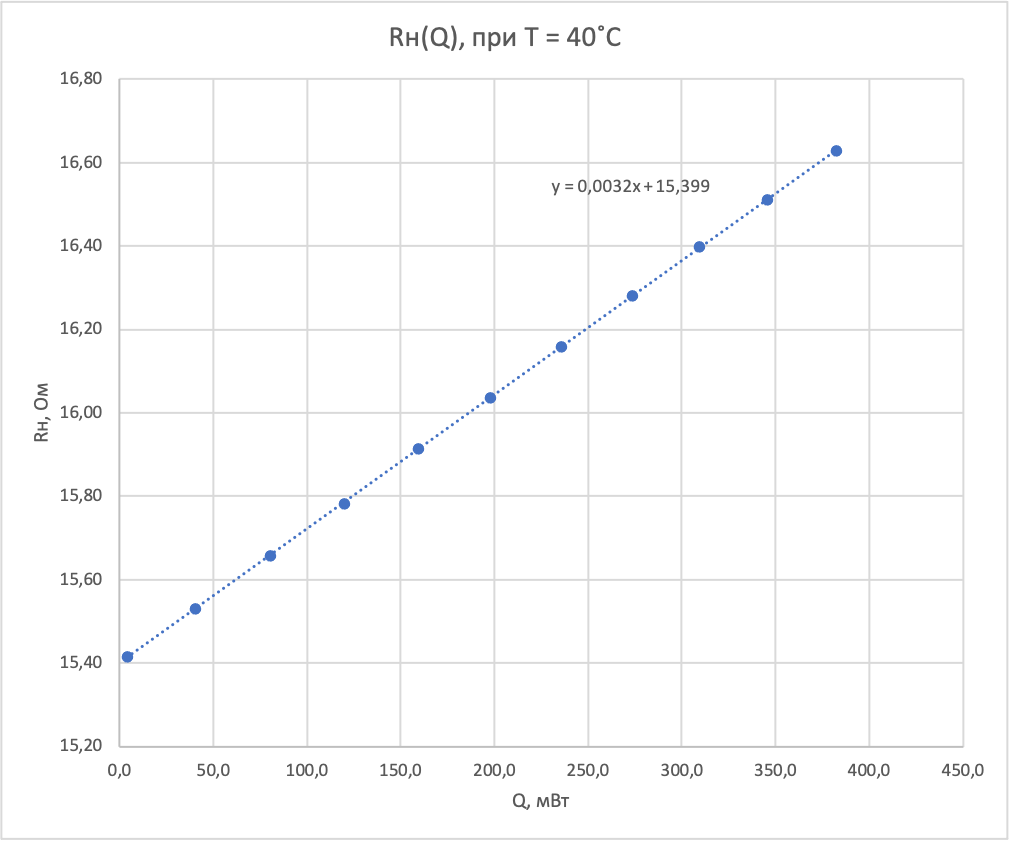
\includegraphics[width=\linewidth]{images/ch3.png}    
        \end{minipage}
        
    \end{table}
    
    \begin{table}
        
        \begin{minipage}[ht]{0.47\linewidth}
            \begin{tabular}{|c|c|c|c|c|}
                \hline
                \multicolumn{5}{|c|}{$T = 50^\circ C$} \\
                \hline
                $R_М$, Ом & $U_1$, мВ & $U_2$, мВ & $Q$, мВт & $R_н$, Ом \\
                \hline
                0 & 1493 & 2546 & 380,1 & 17,05 \\
                \hline
                1,4 & 1425 & 2414 & 344,0 & 16,94 \\
                \hline
                3 & 1355 & 2278 & 308,7 & 16,81 \\
                \hline
                4,9 & 1278 & 2137 & 273,1 & 16,72 \\
                \hline
                7,3 & 1192 & 1979 & 235,9 & 16,60 \\
                \hline
                10,4 & 1097 & 1807 & 198,2 & 16,47 \\
                \hline
                14,5 & 990,2 & 1619 & 160,3 & 16,35 \\
                \hline
                20,6 & 864,0 & 1403 & 121,2 & 16,24 \\
                \hline
                30,9 & 710,4 & 1144 & 81,27 & 16,10 \\
                \hline
                54,1 & 506,1 & 808,8 & 40,93 & 15,98 \\
                \hline
                225 & 161,8 & 256,5 & 4,150 & 15,85 \\
                \hline
            \end{tabular}
        \end{minipage}
        \hfill
        \begin{minipage}[ht]{0.47\linewidth}
            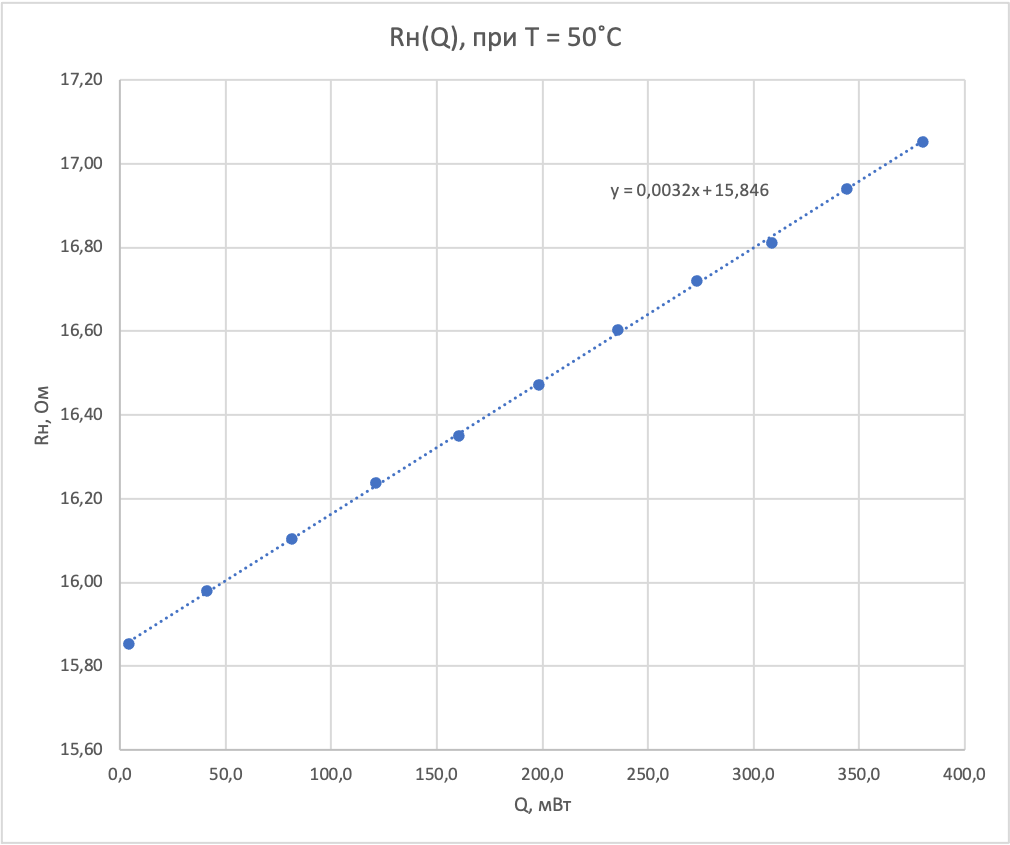
\includegraphics[width=\linewidth]{images/ch4.png}
        \end{minipage}
        
        \vspace{1cm}
        
        \begin{minipage}[ht]{0.47\linewidth}
            \begin{tabular}{|c|c|c|c|c|}
                \hline
                \multicolumn{5}{|c|}{$T = 60^\circ C$} \\
                \hline
                $R_М$, Ом & $U_1$, мВ & $U_2$, мВ & $Q$, мВт & $R_н$, Ом \\
                \hline
                0 & 1470 & 2570 & 377,8 & 17,48 \\
                \hline
                1,4 & 1403 & 2438 & 342,1 & 17,38 \\
                \hline
                3 & 1335 & 2305 & 307,7 & 17,27 \\
                \hline
                4,9 & 1260 & 2164 & 272,7 & 17,17 \\
                \hline
                7,3 & 1177 & 2007 & 236,2 & 17,05 \\
                \hline
                10,4 & 1083 & 1835 & 198,7 & 16,94 \\
                \hline
                14,5 & 979,0 & 1647 & 161,2 & 16,82 \\
                \hline
                20,6 & 855,8 & 1429 & 122,3 & 16,70 \\
                \hline
                30,9 & 704,6 & 1168 & 82,30 & 16,58 \\
                \hline
                54,1 & 503,1 & 827,6 & 41,64 & 16,45 \\
                \hline
                225 & 161,4 & 263,6 & 4,255 & 16,33 \\
                \hline
            \end{tabular}
        \end{minipage}
        \hfill
        \begin{minipage}[ht]{0.47\linewidth}
            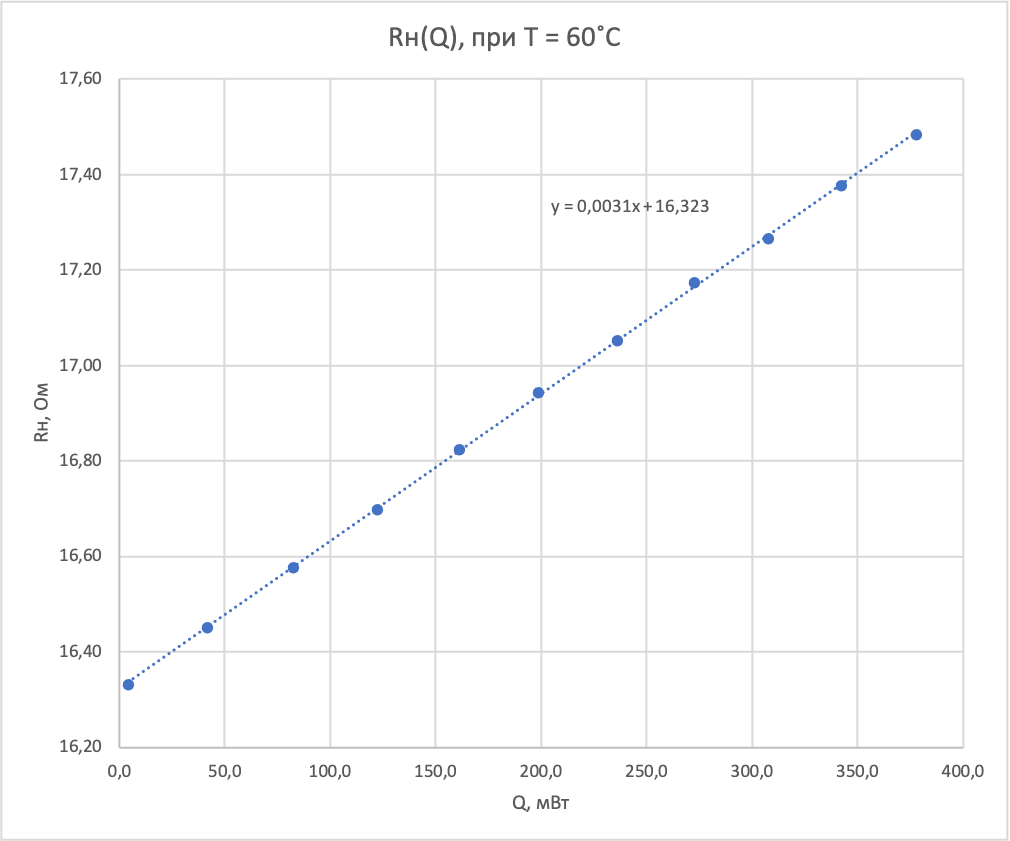
\includegraphics[width=\linewidth]{images/ch5.png}
        \end{minipage}
        
        \caption{Нагрузочные кривые}
        \label{table2}
    \end{table}
    
    \newpage
    
    \begin{center}
        {\Large {\bf Обработка результатов измерений}}
    \end{center}
    
    \begin{enumerate}
    
        \item[1.] Пользуясь данными графиков из табл. \ref{table2}, найдём значения $R_0$: $R_н$ при $Q = 0$ Вт (это значения $R_н$ при температуре равной температуре термостата) и коэффициенты наклона графиков $dR / dQ$. Рассчитаем также погрешности полученных значений. Погрешности будем считать по следующим формулам:
        \begin{equation}
            \sigma_{dR / dQ} = \sqrt{(\sigma_{dR / dQ}^{случ})^2 + (\sigma_{dR / dQ}^{приб})^2},
        \end{equation}
        \begin{equation}
            \sigma_{dR / dQ}^{случ} = \frac{1}{\sqrt{11}} \sqrt{\frac{\langle R^2 \rangle - \langle R \rangle^2}{\langle Q^2 \rangle - \langle Q \rangle^2} - (\frac{dR}{dQ})^2},
        \end{equation}
        \begin{equation}
            \varepsilon_{dR / dQ}^{приб} = \varepsilon_{Q_2 - Q_1},
        \end{equation}
        \begin{equation}
            \sigma_{Q_2 - Q_1} = \sqrt{\sigma_{Q_1}^2 + \sigma_{Q_2}^2},
        \end{equation}
        \begin{equation}
            \varepsilon_Q = \sqrt{4 \cdot \varepsilon_{U_2}^2 + \varepsilon_{U_1}^2}, \text{ } \varepsilon_{U_2} = \varepsilon_{U_1} = \varepsilon_{U} \Rightarrow \varepsilon_Q = \sqrt{5} \cdot \varepsilon_{U}.
        \end{equation}
        Полученные значения $dR / dQ$ и их погрешности занесём в табл. \ref{table3}.
        
        \begin{table}[ht]
            \centering
            \captionsetup{justification=centering, margin=2cm}
            \begin{tabular}{|c|c|c|c|}
                \hline
                $T$, $^\circ C$ & $dR / dQ$, $Ом / Вт$ & $\sigma_{dR / dQ}$, $Ом / Вт$ & $\varepsilon_{dR / dQ}$, \% \\
                \hline
                22 & 3,34 & 0,02 & 0,5 \\
                \hline
                30 & 3,26 & 0,01 & 0,3 \\
                \hline
                40 & 3,22 & 0,01 & 0,3 \\
                \hline
                50 & 3,17 & 0,02 & 0,6 \\
                \hline
                60 & 3,09 & 0,01 & 0,5 \\
                \hline
            \end{tabular}
            \caption{Коэффициенты наклона $dR / dQ$ нагрузочных кривых и их погрешности при данных температурах $T$}
            \label{table3}
        \end{table}
        
        \item[2.] Занесём полученные в п. 1 значения $R_0$ в табл. \ref{table4}. Построим график зависимости сопротивления нити от её температуры $R_0(T)$ (рис. \ref{pic4}).
        
        \begin{figure}[ht]
            \centering
            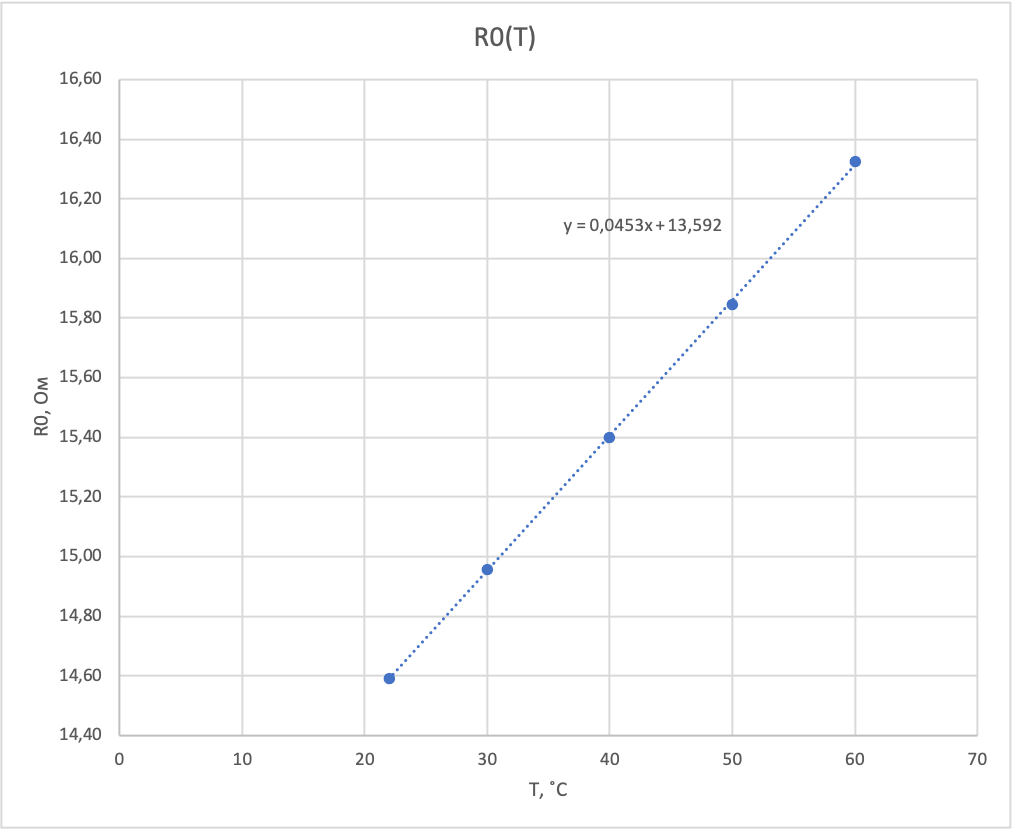
\includegraphics[width=0.55\linewidth]{images/R(T).png}
            \caption{График зависимости $R_0$ от $T$}
            \label{pic4}
        \end{figure}
        
        \begin{table}[ht]
            \centering
            \begin{tabular}{|c|c|c|c|c|c|}
                \hline
                $T$, $^\circ C$ & 22 & 30 & 40 & 50 & 60 \\
                \hline
                $R_0$, Ом & 14,59 & 14,96 & 15,40 & 15,85 & 16,32 \\
                \hline
            \end{tabular}
            \caption{Значения $R_0$ при данных температурах $T$}
            \label{table4}
        \end{table}
        
        Рассчитаем коэффициент наклона графика $dR / dT$ и его погрешность. При подсчёте погрешности воспользуемся следующими формулами:
        \begin{equation}
            \sigma_{dR / dT} = \sqrt{(\sigma_{dR / dT}^{случ})^2 + (\sigma_{dR / dT}^{приб})^2},
        \end{equation}
        \begin{equation}
            \sigma_{dR / dT}^{случ} = \frac{1}{\sqrt{5}} \sqrt{\frac{\langle R^2 \rangle - \langle R \rangle^2}{\langle T^2 \rangle - \langle T \rangle^2} - (\frac{dR}{dT})^2},
        \end{equation}
        \begin{equation}
            \varepsilon_{dR / dT}^{приб} = \varepsilon_{T_2 - T_1},
        \end{equation}
        \begin{equation}
            \sigma_{T_2 - T_1} = \sqrt{(\sigma_{T_1})^2 + (\sigma_{T_2})^2} = \sqrt{2} \cdot \sigma_T.
        \end{equation}
        Окончательно получим:
        \begin{equation}
            \frac{dR}{dT} = (4,53 \pm 0,03) \cdot 10^{-2} \text{ } \frac{Ом}{К}.
        \end{equation}
        
        \item[3.] Зная значения $dR / dQ$ и $dR / dT$, рассчитаем:
        \begin{equation}
            \frac{dQ}{d(\Delta T)} = \frac{dR}{dT} / \frac{dR}{dQ},
        \end{equation}
        для различных температур $T$. Посчитаем также погрешности полученных значений по следующей формуле:
        \begin{equation}
            \varepsilon_{dQ / d(\Delta T)} = \sqrt{(\varepsilon_{dR / dT})^2 + (\varepsilon_{dR / dQ})^2}.
        \end{equation}
        Результаты занесём в табл. \ref{table5}.
        
        Зная значения $dQ / d(\Delta T)$, по формуле \eqref{fifth} найдём значения коэффициента теплопроводности воздуха при температурах $T$:
        \begin{equation}
            k = \frac{Q}{\Delta T} \cdot \frac{ln \frac{r_0}{r_1}}{2 \pi L}.
        \end{equation}
        Рассчитаем погрешность $k$ по следующей формуле:
        \begin{equation}
            \sigma_k^2 = (\frac{\partial k}{\partial (Q / \Delta T)})^2 \cdot \sigma_{Q / \Delta T}^2 + (\frac{\partial k}{\partial r_0})^2 \cdot \sigma_{r_0}^2 + (\frac{\partial k}{\partial r_1})^2 \cdot \sigma_{r_1}^2 + (\frac{\partial k}{\partial L})^2 \cdot \sigma_{L}^2.
        \end{equation}
        Результаты занесём в табл. \ref{table5}.
        
        \newpage
        
        \begin{table}[ht]
            \centering
            
            \begin{tabular}{|c|c|c|c|}
                \hline
                $T$,  $^\circ C$ & $dQ / d(\Delta T)$, $10^{-2} \cdot Вт / К$ & $\sigma_{dQ / d(\Delta T)}$, $10^{-2} \cdot Вт / К$ & $\varepsilon_{dQ / d(\Delta T)}$, \% \\
                \hline
                22 & 1,36 & 0,01 & 0,9 \\
                \hline
                30 & 1,39 & 0,01 & 0,8 \\
                \hline
                40 & 1,41 & 0,01 & 0,8 \\
                \hline
                50 & 1,43 & 0,01 & 0,9 \\
                \hline
                60 & 1,47 & 0,01 & 0,9 \\
                \hline
            \end{tabular}
            
            \vspace{0.5cm}
            
            \begin{tabular}{|c|c|c|c|}
                \hline
                $T$, $^\circ C$ & $k$, $Дж / (К \cdot мм)$ & $\sigma_k$, $Дж / (К \cdot мм)$ & $\varepsilon_k$, \% \\
                \hline
                22 & 30,8 & 0,3 & 1 \\
                \hline
                30 & 31,5 & 0,3 & 1 \\
                \hline
                40 & 31,9 & 0,3 & 1 \\
                \hline
                50 & 32,4 & 0,3 & 1 \\
                \hline
                60 & 33,3 & 0,3 & 1 \\
                \hline
            \end{tabular}
            
            \caption{Значения $dQ / d(\Delta T)$ и $k$ при данных $T$}
            \label{table5}
        \end{table}
        
        \item[4.] Пользуясь данными табл. \ref{table5} проведём наилучшую прямую по МНК через точки зависимости коэффициента теплопроводности воздуха $k$ от температуры $T$. Результат представим на рис. \ref{pic5}.
        
        \begin{figure}[ht]
            \centering
            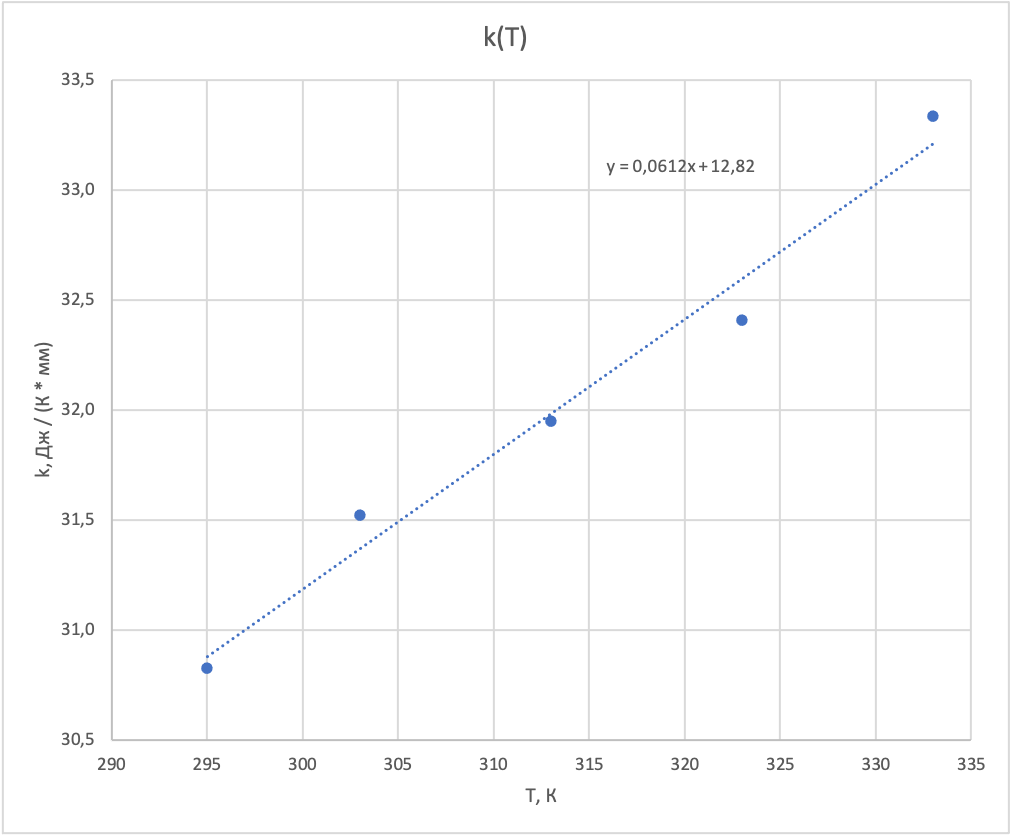
\includegraphics[width=0.6\linewidth]{images/k(T).png}
            \caption{График зависимости $k$ от $T$}
            \label{pic5}
        \end{figure}
        
        Предполагая, что $k$ степенным образом зависит от абсолютной температуры $T$: $k \propto T^{\beta}$, построим график зависимости $lnk$ от $lnT$ и определим из него показатель степени $\beta$. Результаты представим в табл. \ref{table6} и рис. \ref{pic6}.
        
        \vspace{0.7cm}
        
        \begin{table}[h!]
            \centering
            \begin{tabular}{|c|c|c|c|c|c|}
                \hline
                $lnT$, К & 5,69 & 5,71 & 5,75 & 5,78 & 5,81 \\
                \hline
                $lnk$, $Дж / (К \cdot м)$ & -3,48 & -3,46 & -3,44 & 3,43 & -3,40 \\
                \hline
            \end{tabular}
            \caption{$lnT$ и $lnk$}
            \label{table6}
        \end{table}
        
        \begin{figure}[ht]
            \centering
            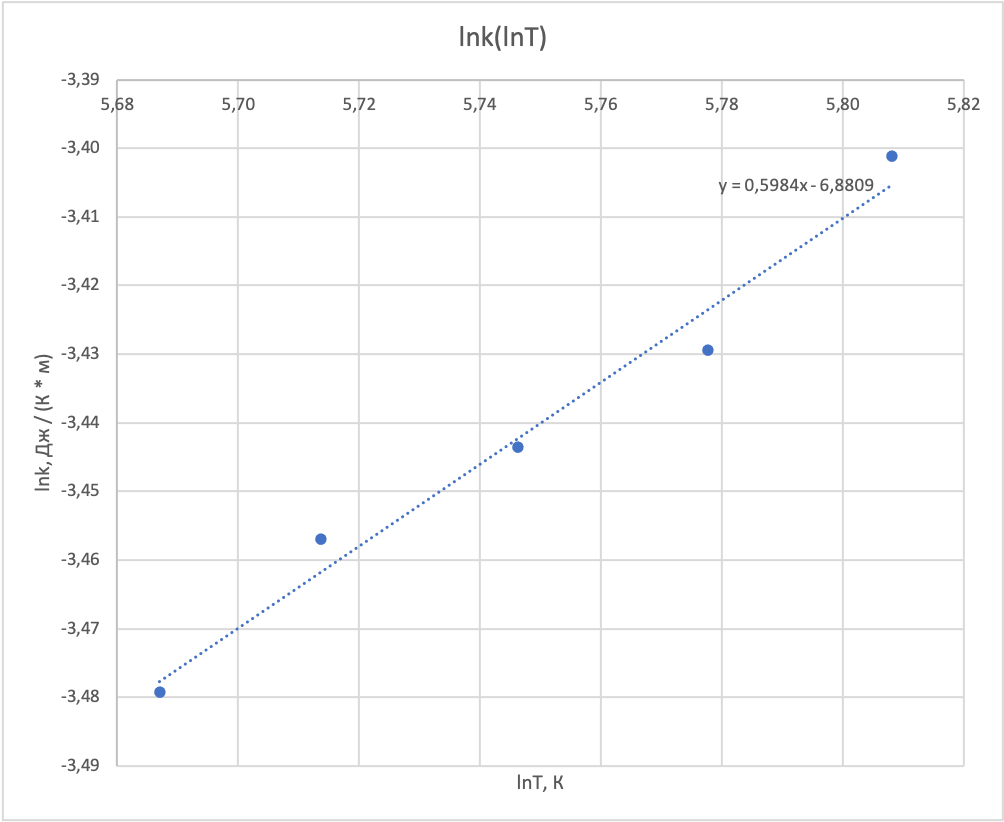
\includegraphics[width=0.6\linewidth]{images/lnk(lnT).png}
            \caption{График зависимости $lnk$ от $lnT$}
            \label{pic6}
        \end{figure}
        
        Коэффициент наклона этого графика: $\beta = 0,6$ $Дж / м$. Погрешность $\beta$ посчитаем по следующей формуле:
        \begin{equation}
            \sigma_{\beta}^{случ} = \frac{1}{\sqrt{5}} \sqrt{\frac{\langle ln(k)^2 \rangle - \langle ln(k) \rangle^2}{\langle ln(T)^2 \rangle - \langle ln(T) \rangle^2} - \beta^2}.
        \end{equation}
        Приборная погрешность мала, поэтому ей можно пренебречь, тогда: $\sigma_{\beta}^{случ} = \sigma_{\beta}$.
        
        В итоге:
        \begin{equation}
            \beta = (0,60 \pm 0,04) \text{ } \frac{Дж}{м}.
        \end{equation}
        
    \end{enumerate}
    
    \vspace{0.5cm}
    
    \begin{center}
        {\Large {\bf Вывод}}
    \end{center}
    
    \noindent В ходе данной работы мы измерили коэффициент теплопроводности воздуха и исследовали зависимость коэффициента теплопроводности от температуры. Маленькие погрешности измерений связаны с маленькими погрешностями приборов, с помощью которых проводились измерения, и точными графиками. Несмотря на это значение коэффициента теплопроводности сходится с табличным только по порядку. Это может быть связано с различными пренебрежениями, сделанными нами в нашей физической модели.

\end{document}